\documentclass{article}

% Language setting
% Replace `english' with e.g. `spanish' to change the document language
\usepackage{polski}
\usepackage[utf8]{inputenc}
\usepackage[T1]{fontenc}
\usepackage{lmodern}

% Set page size and margins
% Replace `letterpaper' with `a4paper' for UK/EU standard size
\usepackage[letterpaper,top=2cm,bottom=2cm,left=3cm,right=3cm,marginparwidth=1.75cm]{geometry}

% Useful packages
\usepackage{amsmath}
\usepackage{graphicx}
\usepackage[colorlinks=true, allcolors=black]{hyperref}
\usepackage{fancyhdr} 
\usepackage{lastpage}
\usepackage{ifthen}
\usepackage{hyperref}

\title{Specyfikacja implementacyjna programu CGrafy}
\author{Szymon Posiadała i Jordan Parviainen}
\date{20.03.2022r.}

\pagestyle{fancy}
\fancyhf{}

\lhead{\ifthenelse{\value{page}=1}{}{Specyfikacja implementacyjna CGrafy}}
\rhead{\ifthenelse{\value{page}=1}{}{Szymon Posiadała i Jordan Parviainen}}
\cfoot{Strona \thepage \hspace{1pt} z \pageref{LastPage}}

\fancypagestyle{firststyle}
{
    \renewcommand{\headrulewidth}{0pt}
    \cfoot{Strona \thepage \hspace{1pt} z \pageref{LastPage}}
}

\setlength{\belowcaptionskip}{20pt}

\begin{document}
\maketitle

\thispagestyle{firststyle}

\section{Wstęp}
Opis programu, jego funkcji, jak i celu jego powstania można znaleźć w Specyfikacji funkcjonalnej.

\section{Wymagania technologiczne}
Program ma być napisany w języku C w standardzie ANSI-C (C99). Użyty powinien być kompilator GNU Compiler w wersji 7.3.0. Do kompilacji i testów powinno się używać programu \texttt{Make}. Narzędziem do kontroli wersji będzie program \texttt{git}. Repozytorium projektu jest przechowywane na stronie Projektor (\texttt{https://projektor.ee.pw.edu.pl/}). Program musi działać na maszynie Politechniki Warszawskiej o nazwie "jimp". Program ma działać w interfejsie tekstowym.

\section{Wejście i wyjście}
Wejście i wyjście jest szczegółowo opisane w Specyfikacji funkcjonalnej tego projektu.

\section{Opis modułów i struktur danych}
\begin{figure}[h]
    \centering
    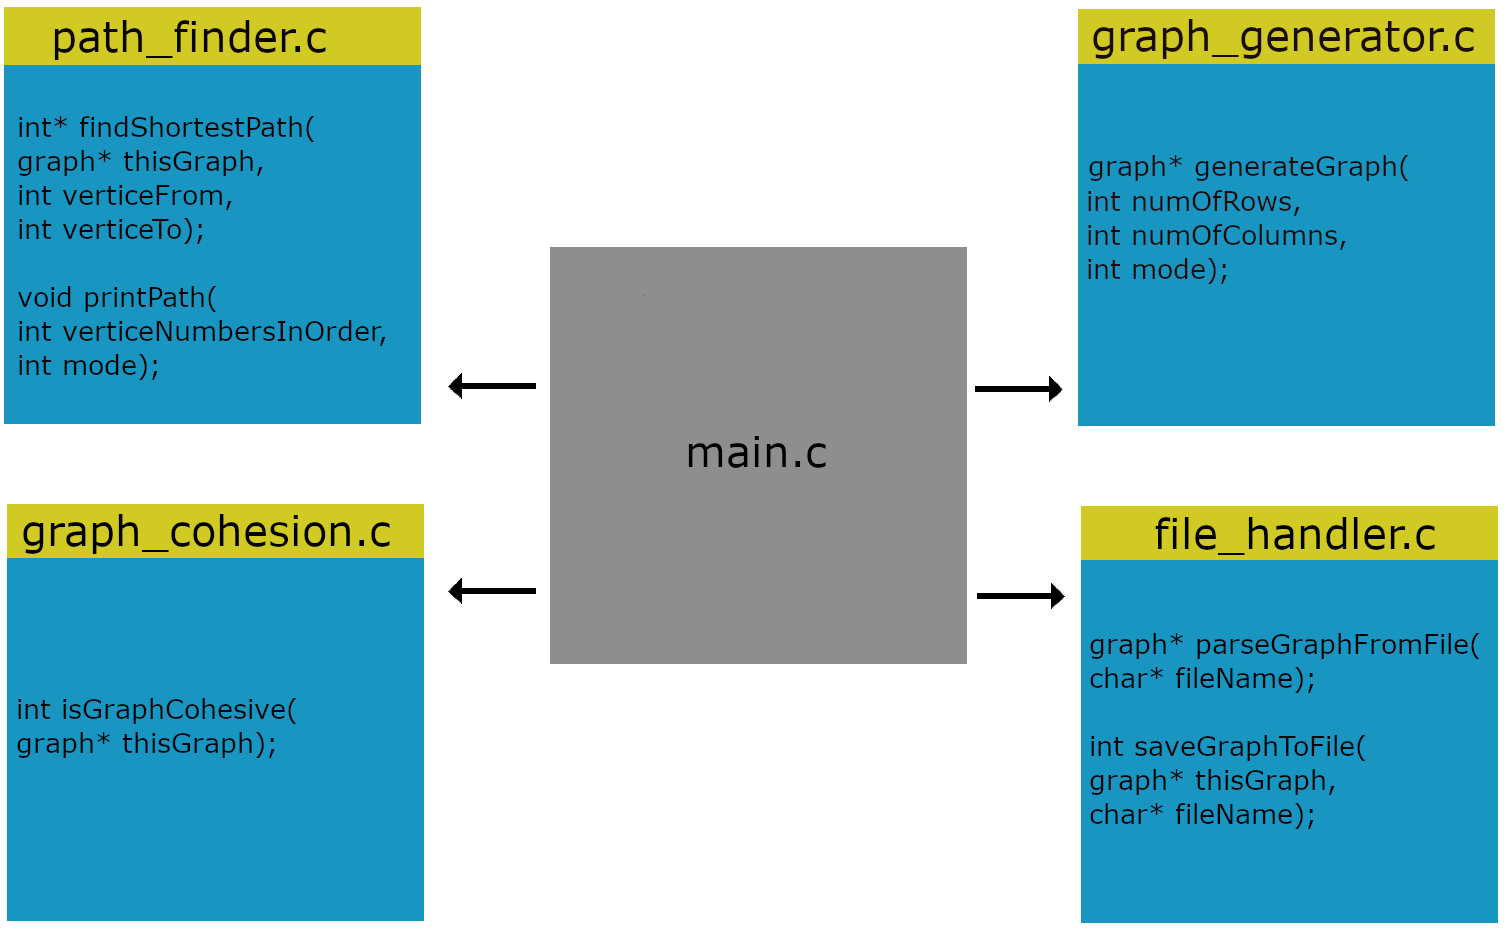
\includegraphics[scale=0.4]{si}
    \caption{Schemat modułów programu}
    \label{fig:schemat}
\end{figure}
\subsection{Struktury danych} 
Główną daną w programie, która będzie przekazywana do i zwracana przez jego główne funkcje w~modułach to struktura o nazwie \texttt{graph}. Przedstawia się ona następująco w pseudokodzie:\\
\texttt{struct graph\{} \\
\texttt{int numberOfColumns;} -- liczba kolumn siatki grafu\\
\texttt{int numberOfRows;} -- liczba wierszy siatki grafu\\
\texttt{vertice vertices[numberOfColumns*numberOfRows];} -- tablica przechowująca wierzchołki opisane za pomocą struktury vertice, która jest przedstawiona poniżej\\
\texttt{\}} \\
Struktura opisująca wierzchołek: \\
\texttt{struct vertice\{ } \\
\texttt{int verticeNumber;} -- identyfikator wierzchołka zgodnie z numeracją przedstawioną w Specyfikacji funkcjonalnej \\
\texttt{double weightLeft;} -- waga połączenia tego wierzchołka do wierzchołka leżącego bezpośrednio po jego lewej stronie w siatce grafu; wartość \texttt{0} jeśli tego połączenia nie ma \\
\texttt{double weightRight;} -- waga połączenia tego wierzchołka do wierzchołka leżącego bezpośrednio po jego prawej stronie w siatce grafu; wartość \texttt{0} jeśli tego połączenia nie ma \\
\texttt{double weightUp;} -- waga połączenia tego wierzchołka do wierzchołka leżącego bezpośrednio nad nim w siatce grafu; wartość \texttt{0} jeśli tego połączenia nie ma \\
\texttt{double weightDown;} -- waga połączenia tego wierzchołka do wierzchołka leżącego bezpośrednio pod nim w siatce grafu; wartość \texttt{0} jeśli tego połączenia nie ma \\
\texttt{ \} } \\
\subsection{Moduły}
\label{sec:moduly}
\begin{itemize}
    \item \texttt{main.c} \\
    Główny moduł, steruje pracą programu, a jego funkcja \texttt{int main(int argc, char* args[])} stanowi punkt wejścia programu, od którego rozpoczyna się jego wykonywanie. W module tym przetwarzane są argumenty wejściowe programu z linii poleceń, jak i wywoływane są funkcje z~pozostałych modułów programu.
    \item \texttt{path\_finder.c} \\
    Moduł ten realizuje funkcję znajdowania najkrótszej ścieżki w grafie pomiędzy podanymi wierzchołkami oraz jej wypisywanie. \\
    Najważniejsze funkcje:
    \begin{itemize}
        \item \texttt{int* findShortestPath(graph* thisGraph, int verticeFrom, int verticeTo)} \\
        Funkcja znajdująca najkrótszą drogę pomiędzy wierzchołkami oznaczonymi numerami \texttt{verticeFrom} a \texttt{verticeTo} w grafie przekazanym w postaci struktury \texttt{graph}.
        Funkcja zwraca wskaźnik na tablicę z kolejnymi numerami wierzchołków składającymi się na drogę.
        \item \texttt{void printPath(int* verticeNumbersInOrder, int mode)} \\
        Funkcja ta wypisuje na ekran ścieżkę obliczoną przez funkcję. \texttt{findShortestPath()} w formacie opisanym w Specyfikacji Funkcjonalnej. Są możliwe dwa tryby wypisywania ścieżki, podstawowy i rozszerzony, co jest przekazywane za pomocą argumentu \texttt{mode}.
    \end{itemize}
    \item \texttt{graph\_generator.c} \\
    Moduł ten realizuje generowanie grafu. \\
    Najważniejsza funkcja: \\
    \texttt{graph* generateGraph(int numOfRows, int numOfColumns, int mode)} \\
    Przyjmuje ona wielkość grafu w postaci liczby wierszy i kolumn oraz jeden z 3 trybów generowania grafu, po szczegóły odsyłam do Specyfikacji Funkcjonalnej. Funkcja zwraca wskaźnik na strukturę \texttt{graph}.
    \item \texttt{file\_handler.c} \\
    Moduł ten obsługuje operacje zapisu grafu do pliku, jak i jego odczytu z pliku. \\ 
    Najważniejsze funkcje:
    \begin{itemize}
        \item \texttt{graph* parseGraphFromFile(char* fileName)} \\
        Funkcja zczytuje graf z pliku w formacie podanym w Specyfikacji funkcjonalnej, zwraca wskaźnik na strukturę \texttt{graph} utworzoną według informacji w pliku.
        \item \texttt{int saveGraphToFile(graph* thisGraph, char* fileName)} \\
        Funkcja zapisuje graf do pliku i zwraca \texttt{1}, jeśli operacja się powiodła i \texttt{0}, jeśli nie.
    \end{itemize}
    \item \texttt{graph\_cohesion.c} \\
    Moduł ten odpowiedzialny jest za sprawdzanie spójności grafu. \\
    Najważniejsza funkcja: \\
    \texttt{int isGraphCohesive(graph* thisGraph)} \\
    Funkcja przyjmuje wskaźnik na strukturę \texttt{graph} i zwraca \texttt{1}, jeśli graf jest spójny i \texttt{0}, jeśli graf nie jest spójny.
\end{itemize}

\section{Testowanie}
Do każdego modułu powinien zostać napisany odpowiadający mu test sprawdzający poprawność działania jego najważniejszych funkcji, czyli tych opisanych w sekcji tego dokumentu \hyperref[sec:moduly]{"Moduły"}. Testy i~dane testowe powinny być w taki sposób konstruowane, żeby proces testowania mógł być zautomatyzowany w programie \texttt{Make}. Należy będzie stworzyć pliki z wzorcowym wyjściem testów i dodać regułę w \texttt{Makefile} porównującą wyjście programu testowego do wyjścia wzorcowego i zwracać komunikat o~powodzeniu lub nie.\\ 
Oprócz typowych zastosowań tych funkcji powinno być testowane ich zachowanie w przypadku błędnych danych wejściowych i przypadków brzegowych.
Analogicznie powinny zostać stworzone testy do całego skończonego programu. Szczególne przypadki testowe to m.in. niepoprawny format argumentów wywołania, zły format pliku wejściowego, zbyt duża liczba kolumn i wierszy w generowanych i~zczytywanych grafach.

\section{Praktyki projektowe}

\subsection{Konwencje notacyjne w kodzie}
Wszelkie nazwy w kodzie, jak i komentarze mają być pisane w języku angielskim. Nazwy funkcji i~zmiennych powinny być pisane zgodnie z konwencją notacyjną \texttt{camelCase}, pierwsza litera powinna być mała. Nazwy modułów z rozszerzeniem \texttt{.c} oraz plików nagłówkowych z rozszerzeniem \texttt{.h} powinny być pisane z użyciem konwencji notacyjnej \texttt{snake\_case}.

\subsection{Sposób pracy z repozytorium}
Każdy członek zespołu rozpoczynający pracę nad nową, oddzieloną funkcyjnie częścią kodu (moduł, główna funkcja modułu) winien utworzyć nową gałąź w repozytorium i pracować na niej do momentu doprowadzenia danej części programu do stanu użyteczności. Wtedy należy dokonać złączenia gałęzi z~
główną i w przypadku konfliktów rozwiązać je w porozumieniu z innymi członkami zespołu. W~przypadku poprawek lub innych przypadków edytowania kodu dopuszcza się dowolność sposobu pracy z~repozytorium, jednak zawsze należy mieć na uwadze przejrzystość prac nad kodem dla wszystkich członków zespołu. Wiadomości dołączone do commitów powinny ściśle opisywać zmiany dokonane w~danym commicie.
\end{document}